\chapter{Atoomorbitalen: vormen, energieën en afmetingen}\label{ch:b2:atomic-orbitals}

Een waterstofatoom heeft geen rand: zijn elektron kan op elke afstand van de kern
gevonden worden, met een waarschijnlijkheid die snel afneemt maar nooit nul
wordt. Toch hebben atomen een afmeting, en een natriumatoom is ongeveer tweemaal zo breed als een
chlooratoom, hoewel het minder elektronen bevat. Het deel van jaar~1 benoemde de
toestanden van een elektron met drie kwantumgetallen; hier wordt elk ervan een
functie van de plaats, met een vorm, knopen, tekens en een afmeting, en een eenvoudige verzameling
regels maakt er orbitaalenergieën van voor elk atoom. Deze vormen en tekens
zijn wat de volgende vier hoofdstukken tot molecuulorbitalen combineren.

\begin{recall}
Het deel van jaar~1: kwantumgetallen $n$, $l$, $m_l$, $m_s$; atoomorbitalen als de
toestanden $(n, l, m_l)$; schillen en subschillen; afscherming en effectieve kernlading
(kwalitatief); elektronenconfiguraties; de niveaus van waterstof,
$-E_R/n^2$ met $E_R = \qty{13.6}{eV}$. Uit de natuurkunde: de \omterm{def:b2:atomic-orbitals:wavefunction}{golffunctie}, waarvan de
kwadratische modulus een \omterm{def:b2:atomic-orbitals:wavefunction}{waarschijnlijkheidsdichtheid} is.
\end{recall}

\section{De golffuncties van het waterstofatoom}

\begin{definition}[Golffunctie]\label{def:b2:atomic-orbitals:wavefunction}
De toestand van een elektron wordt beschreven door een \emph{golffunctie}\index{golffunctie}
$\psi(x, y, z)$; $|\psi|^2$ is haar \emph{waarschijnlijkheidsdichtheid}\index{waarschijnlijkheidsdichtheid}:
de waarschijnlijkheid om het elektron te vinden in een klein volume $dV$ rond
een punt is $|\psi|^2\,dV$, en $\int|\psi|^2\,dV = 1$ over de hele ruimte (de functie
is genormeerd). Een atoomorbitaal is de golffunctie van één elektron in een
atoom.
\end{definition}

\begin{definition}[Radiaal deel en hoekdeel]\label{def:b2:atomic-orbitals:radial-angular}
In bolcoördinaten $(r, \theta, \varphi)$ rond de kern ontbinden de orbitalen van
een waterstofachtig atoom zich als $\psi_{nlm}(r, \theta, \varphi) = R_{nl}(r)\,
Y_{lm}(\theta, \varphi)$: het \emph{radiaal deel}\index{radiaal deel} $R_{nl}$ hangt af
van $n$ en $l$, het \emph{hoekdeel}\index{hoekdeel} $Y_{lm}$ alleen van $l$ en
$m_l$.
\end{definition}

\begin{theorem}[De waterstofachtige orbitalen]\label{thm:b2:atomic-orbitals:hydrogen}
Voor een atoom met één elektron en kernlading $Ze$, met $\rho = Zr/a_0$ en $a_0 =
\qty{52.9}{pm}$ de bohrstraal, zijn de radiale delen voor $n \leq 3$, in eenheden van
$(Z/a_0)^{3/2}$:
\[
\begin{array}{ll}
  R_{1s} = 2\,\mathrm e^{-\rho} &
  R_{2s} = \dfrac{1}{2\sqrt2}\,(2 - \rho)\,\mathrm e^{-\rho/2} \\[2ex]
  R_{2p} = \dfrac{1}{2\sqrt6}\,\rho\,\mathrm e^{-\rho/2} &
  R_{3s} = \dfrac{2}{81\sqrt3}\,(27 - 18\rho + 2\rho^2)\,\mathrm e^{-\rho/3} \\[2ex]
  R_{3p} = \dfrac{4}{81\sqrt6}\,(6\rho - \rho^2)\,\mathrm e^{-\rho/3} &
  R_{3d} = \dfrac{4}{81\sqrt{30}}\,\rho^2\,\mathrm e^{-\rho/3}
\end{array}
\]
en de reële hoekdelen zijn $Y_s = 1/\sqrt{4\pi}$; $Y_{p_x}, Y_{p_y}, Y_{p_z} =
\sqrt{3/(4\pi)}\,(x, y, z)/r$; $Y_{d_{xy}} = \sqrt{15/(4\pi)}\,xy/r^2$ (en evenzo
$xz$, $yz$), $Y_{d_{x^2-y^2}} = \sqrt{15/(16\pi)}\,(x^2 - y^2)/r^2$, $Y_{d_{z^2}} =
\sqrt{5/(16\pi)}\,(3z^2 - r^2)/r^2$. Hun energieën zijn $E_n = -Z^2E_R/n^2$.
% ledger: const:a0, const:RyhcEV
\end{theorem}

\admitted

Deze functies zijn de oplossingen van de schrödingervergelijking voor één elektron
en één kern, die in het deel van jaar~3 gevonden worden. De reële $p$- en $d$-functies zijn
combinaties van de complexe functies met label $m_l$; ze wijzen langs de assen en
worden gebruikt om bindingen op te bouwen.

\begin{omfigure}
\begin{minipage}[t]{0.27\linewidth}\vspace{0pt}
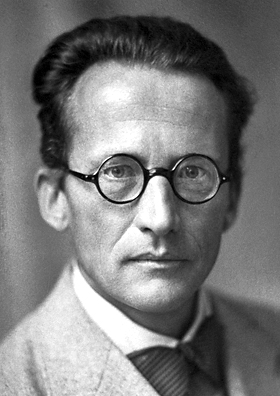
\includegraphics[width=\linewidth]{images/book3/schrodinger.jpg}
\end{minipage}\hfill
\begin{minipage}[t]{0.69\linewidth}\vspace{0pt}
{\small Erwin Schrödinger, die in 1926 de golfvergelijking opstelde waarvan de
oplossingen voor het waterstofatoom de orbitalen van dit hoofdstuk zijn, en die er
de energieniveaus uit terugvond die Bohr had gepostuleerd. Hij deelde in 1933 de
Nobelprijs voor Natuurkunde. (Foto: Nobelstichting, publiek domein,
Wikimedia Commons.)}
\end{minipage}
\end{omfigure}

\section{Het radiale deel}

De waarschijnlijkheid om het elektron tussen de bollen met stralen $r$ en $r +
dr$ te vinden, is $|\psi|^2$ geïntegreerd over de schil met volume $4\pi r^2\,dr$; voor elke
orbitaal is dat, na integratie over de hoeken, $r^2R^2\,dr$.

\begin{definition}[Radiale verdeling]\label{def:b2:atomic-orbitals:radial-distribution}
De \emph{radiale verdelingsfunctie}\index{radiale verdelingsfunctie} van
een orbitaal is $P(r) = r^2R_{nl}(r)^2$: $P(r)\,dr$ is de waarschijnlijkheid dat het
elektron zich tussen $r$ en $r + dr$ van de kern bevindt. De \emph{meest waarschijnlijke
straal}\index{meest waarschijnlijke straal} is de waarde van $r$ bij haar grootste maximum.
\end{definition}

\begin{proposition}[Normering van 1s]\label{prop:b2:atomic-orbitals:normalised}
$\int_0^\infty P_{1s}(r)\,dr = 1$.
\end{proposition}

\begin{proof}
Met $Z = 1$ en $r$ in eenheden van $a_0$ is $P_{1s} = 4r^2\mathrm e^{-2r}$. Tweemaal partieel integreren geeft
$\int_0^\infty r^2\mathrm e^{-2r}\,dr = \frac22\int_0^\infty r\,\mathrm e^{-2r}\,dr =
\frac12\int_0^\infty\mathrm e^{-2r}\,dr = \frac14$, en $4 \times \frac14 = 1$.
\end{proof}

\begin{proposition}[Meest waarschijnlijke straal]\label{prop:b2:atomic-orbitals:most-probable}
Voor de 1s-orbitaal is de \omterm{def:b2:atomic-orbitals:radial-distribution}{meest waarschijnlijke straal} $a_0/Z$. Voor een orbitaal met $l =
n - 1$ (1s, 2p, 3d, \dots) is hij $n^2a_0/Z$.
\end{proposition}

\begin{proof}
Voor $l = n - 1$ heeft het \omterm{def:b2:atomic-orbitals:radial-angular}{radiale deel} geen knoop: $R \propto \rho^{n-1}\mathrm e^{-\rho/n}$,
dus $P \propto \rho^{2n}\mathrm e^{-2\rho/n}$ en $d\ln P/d\rho = 2n/\rho - 2/n$, nul
voor $\rho = n^2$, dus $r = n^2a_0/Z$. Met $n = 1$ is $r = a_0/Z$.
\end{proof}

\begin{proposition}[Gemiddelde straal van 1s]\label{prop:b2:atomic-orbitals:mean-radius}
De gemiddelde afstand van een 1s-elektron tot de kern is $\langle r\rangle = 3a_0/(2Z)$,
groter dan zijn \omterm{def:b2:atomic-orbitals:radial-distribution}{meest waarschijnlijke straal}.
\end{proposition}

\begin{proof}
Met $Z = 1$: $\langle r\rangle = \int_0^\infty r\,P(r)\,dr = 4\int_0^\infty r^3\mathrm e^{-2r}
\,dr = 4 \times 3!/2^4 = 3/2$. De verdeling heeft een lange staart bij grote $r$,
die het gemiddelde voorbij het maximum trekt.
\end{proof}

\begin{definition}[Knopen]\label{def:b2:atomic-orbitals:node}
Een \emph{knoopvlak}\index{knoopvlak} van een orbitaal is een oppervlak waarop
de \omterm{def:b2:atomic-orbitals:wavefunction}{golffunctie} nul is en van teken verandert. Het is een \emph{radiale knoop}\index{radiale knoop}
(een bol) wanneer het \omterm{def:b2:atomic-orbitals:radial-angular}{radiale deel} nul wordt, een
\emph{hoekknoop}\index{hoekknoop} (een vlak of een kegel door de kern) wanneer het \omterm{def:b2:atomic-orbitals:radial-angular}{hoekdeel}
nul wordt.
\end{definition}

\begin{proposition}[Knopen tellen]\label{prop:b2:atomic-orbitals:nodes}
Een orbitaal $(n, l)$ heeft $n - l - 1$ radiale knopen en $l$ hoekknopen, $n - 1$ in
totaal.
\end{proposition}

\begin{proof}
Op de functies van \cref{thm:b2:atomic-orbitals:hydrogen}: $R_{2s}$ wordt nul bij
$\rho = 2$, $R_{3s}$ bij de twee wortels van $2\rho^2 - 18\rho + 27$ ($\rho = 1.90$ en $7.10$),
$R_{3p}$ bij $\rho = 6$; $R_{1s}$, $R_{2p}$, $R_{3d}$ worden niet nul. Het \omterm{def:b2:atomic-orbitals:radial-angular}{hoekdeel}
van een p-orbitaal wordt nul op één vlak ($z = 0$ voor $p_z$), dat van een d-orbitaal op twee
vlakken of, voor $d_{z^2}$, op een kegel. Het algemene geval wordt aangenomen.
\end{proof}

\begin{omfigure}
\begin{tikzpicture}
\begin{axis}[width=0.55\linewidth, height=6cm, xmin=0, xmax=24, ymin=0, ymax=0.58,
  axis x line=bottom, axis y line=left, xlabel={$r/a_0$}, ylabel={$P(r)$},
  tick label style={font=\small}, label style={font=\small}, title={\small radiale verdelingen, $Z = 1$}]
\addplot[omThm, thick] table[x=r, y=s1] {figdata/out/bachelor-2-atomic-orbitals-a.dat};
\addplot[omDef, thick] table[x=r, y=s2] {figdata/out/bachelor-2-atomic-orbitals-a.dat};
\addplot[omDef, thick, dashed] table[x=r, y=p2] {figdata/out/bachelor-2-atomic-orbitals-a.dat};
\addplot[omProp, thick] table[x=r, y=s3] {figdata/out/bachelor-2-atomic-orbitals-a.dat};
\addplot[omProp, thick, dashed] table[x=r, y=p3] {figdata/out/bachelor-2-atomic-orbitals-a.dat};
\addplot[omProp, thick, dotted] table[x=r, y=d3] {figdata/out/bachelor-2-atomic-orbitals-a.dat};
\node[font=\scriptsize, omThm, anchor=west] at (axis cs:1.4,0.53) {1s};
\node[font=\scriptsize, omDef, anchor=south] at (axis cs:4.0,0.215) {2p};
\node[font=\scriptsize, omDef, anchor=south west] at (axis cs:6.4,0.17) {2s};
\node[font=\scriptsize, omProp, anchor=south] at (axis cs:10.5,0.12) {3d};
\node[font=\scriptsize, omProp, anchor=west] at (axis cs:17,0.085) {3s, 3p};
\end{axis}
\end{tikzpicture}\hfill
\begin{tikzpicture}
\begin{axis}[width=0.42\linewidth, height=6cm, xmin=0, xmax=20, ymin=-0.12, ymax=0.75,
  axis x line=middle, axis y line=left, xlabel={$r/a_0$}, ylabel={$R$},
  tick label style={font=\small}, label style={font=\small}, title={\small radiale delen}]
\addplot[omDef, thick] table[x=r, y=R2s] {figdata/out/bachelor-2-atomic-orbitals-b.dat};
\addplot[omProp, thick] table[x=r, y=R3s] {figdata/out/bachelor-2-atomic-orbitals-b.dat};
\node[font=\scriptsize, omDef, anchor=west] at (axis cs:0.4,0.62) {$R_{2s}$};
\node[font=\scriptsize, omProp, anchor=west] at (axis cs:0.6,0.30) {$R_{3s}$};
\node[font=\scriptsize, anchor=south west] at (axis cs:3,0.15) {knoop};
\draw[thin, ->] (axis cs:3,0.15) -- (axis cs:2.05,0.01);
\end{axis}
\end{tikzpicture}

{\small Links: radiale verdelingen $P(r) = r^2R^2$ van de orbitalen van waterstof tot
$n = 3$; hoe groter $n$, hoe verder het elektron, en de s-orbitalen hebben
kleine binnenste maxima (penetratie). Rechts: $R_{2s}$ en $R_{3s}$ veranderen van teken bij hun
radiale knopen ($r = 2a_0$; $1.90a_0$ en $7.10a_0$).}
\end{omfigure}

\begin{omfigure}
\begin{tikzpicture}
\begin{axis}[scale only axis, width=0.32\linewidth, height=0.32\linewidth,
  xmin=-6, xmax=6, ymin=-6, ymax=6, axis lines=none, title={\small 1s}]
\addplot[only marks, mark=*, mark size=0.25pt, omDef] table[x=x, y=y] {figdata/out/bachelor-2-atomic-orbitals-c-1s.dat};
\end{axis}
\end{tikzpicture}\hspace{0.12\linewidth}%
\begin{tikzpicture}
\begin{axis}[scale only axis, width=0.32\linewidth, height=0.32\linewidth,
  xmin=-14, xmax=14, ymin=-14, ymax=14, axis lines=none, title={\small 2s}]
\addplot[only marks, mark=*, mark size=0.25pt, omDef] table[x=x, y=y] {figdata/out/bachelor-2-atomic-orbitals-c-2s.dat};
\draw[densely dashed, omThm] (axis cs:0,0) circle[radius=2];
\end{axis}
\end{tikzpicture}

{\small Puntdichtheidsbeelden van de 1s- en 2s-orbitalen van waterstof in een vlak
door de kern: de dichtheid van de punten volgt $|\psi|^2$ (deterministische
bemonstering). De 2s-wolk heeft een lege ring, de \omterm{def:b2:atomic-orbitals:node}{radiale knoop} bij $2a_0$ (gestreept);
de kaders zijn 12 en 28 $a_0$ breed.}
\end{omfigure}

\section{Het hoekdeel}

Het \omterm{def:b2:atomic-orbitals:radial-angular}{hoekdeel} legt de vorm vast. Een s-orbitaal is bolvormig; een p-orbitaal heeft twee
lobben van tegengesteld teken langs haar as, gescheiden door een \omterm{def:b2:atomic-orbitals:node}{knoopvlak}; een d-orbitaal heeft
vier lobben met afwisselend teken (of, voor $d_{z^2}$, twee lobben en een ring). Het teken
van een lob heeft op zichzelf geen fysische betekenis --- $\psi$ en $-\psi$ beschrijven dezelfde
toestand ---, maar de relatieve tekens van twee orbitalen beslissen in het volgende hoofdstuk
of ze tot een binding combineren.

\begin{omfigure}
\begin{tikzpicture}[font=\small]
  \pic at (0,0) {oms={1}};
  \node[below] at (0,-0.75) {s};
  \pic at (2.0,0) {omp={1}{0}};
  \draw[->, black!55, thin] (1.0,0) -- (3.0,0) node[right, font=\tiny] {$x$};
  \node[below] at (2.0,-0.75) {$\mathrm p_x$};
  \pic at (4.2,0) {omp={1}{90}};
  \draw[->, black!55, thin] (4.2,-0.95) -- (4.2,0.95) node[above, font=\tiny] {$z$};
  \node[below] at (4.75,-0.75) {$\mathrm p_z$};
  \pic at (6.6,0) {omdxy}; \node[below] at (6.6,-1.0) {$\mathrm d_{xy}$};
  \pic at (9.0,0) {omdx2y2}; \node[below] at (9.0,-1.0) {$\mathrm d_{x^2-y^2}$};
  \pic at (11.4,0) {omdz2}; \node[below] at (11.4,-1.0) {$\mathrm d_{z^2}$};
\end{tikzpicture}

{\small Reële atoomorbitalen, schematisch: de lobben tonen de gebieden waar $|\psi|$
groot is, gekleurd naar het teken van $\psi$ (blauw positief, oranje negatief). De
orbitalen $\mathrm d_{xz}$ en $\mathrm d_{yz}$ hebben de vorm van $\mathrm d_{xy}$ in
de vlakken die hun namen aangeven.}
\end{omfigure}

\begin{method}[Een orbitaal schetsen uit zijn kwantumgetallen]\label{met:b2:atomic-orbitals:draw-orbital}
\begin{enumerate}
  \item Uit $l$ de vorm: s (bol), p (twee lobben), d (vier lobben, of twee
        lobben en een ring voor $d_{z^2}$); uit het subscript de oriëntatie.
  \item Tel de $l$ hoekknopen (vlakken door de kern) en geef
        aangrenzende lobben tegengestelde tekens.
  \item Tel de $n - l - 1$ radiale knopen: binnenste schillen van tegengesteld teken binnen
        de hoofdlobben (meestal weggelaten in schetsen).
  \item Schaal met $n^2a_0/Z$: hogere $n$, grotere orbitaal; grotere $Z$, kleinere.
\end{enumerate}
\end{method}

\section{Atomen met meer elektronen}

In een atoom met verscheidene elektronen voelt elk elektron de kern, afgeschermd door
de andere. De orbitalen behouden de vormen van die van waterstof, met een effectieve
lading $Z^*$ in plaats van $Z$, en de energie van een subschil hangt nu ook af van $l$,
niet alleen van $n$: een s-elektron, waarvan de radiale verdeling binnenste maxima dicht bij
de kern heeft, wordt minder afgeschermd dan een p-elektron van dezelfde schil, en een p minder
dan een d.

\begin{definition}[Regels van Slater]\label{def:b2:atomic-orbitals:slater}
De \emph{regels van Slater}\index{regels van Slater} schatten de effectieve kernlading
$Z^* = Z - \sigma$ die een elektron voelt. De elektronen worden gegroepeerd als
(1s) (2s, 2p) (3s, 3p) (3d) (4s, 4p) (4d) (4f) (5s, 5p) \dots; de afschermingsconstante
$\sigma$ van een elektron is de som van de bijdragen van de andere
elektronen: 0.35 voor elk ander elektron van dezelfde groep (0.30 binnen 1s);
voor een s- of p-elektron 0.85 voor elk elektron van de schil $n - 1$ en 1.00 voor
elk elektron van lagere schillen; voor een d- of f-elektron 1.00 voor elk elektron
van de groepen onder zijn eigen groep. Hogere groepen dragen niets bij.
\end{definition}

\begin{omfigure}
\small
\renewcommand{\arraystretch}{1.2}
\begin{tabular}{l|ccccc}
bestudeerd elektron & zelfde groep & schil $n - 1$ & lagere schillen & hogere groepen \\ \hline
1s & 0.30 & --- & --- & 0 \\
$n$s, $n$p & 0.35 & 0.85 & 1.00 & 0 \\
$n$d, $n$f & 0.35 & 1.00 & 1.00 & 0 \\
\end{tabular}

\smallskip
{\small Afschermingsconstanten van Slater, per afschermend elektron. De effectieve
hoofdkwantumgetallen zijn $n^* = 1, 2, 3, 3.7, 4.0, 4.2$ voor $n = 1$ tot 6.}
\end{omfigure}

\begin{method}[Een effectieve lading berekenen]\label{met:b2:atomic-orbitals:slater}
\begin{enumerate}
  \item Schrijf de configuratie in de groepen van Slater, in volgorde van $n$, met s en p
        samen en d en f apart.
  \item Kies het elektron; tel 0.35 op voor elk ander elektron van zijn groep.
  \item Tel 0.85 (s- of p-elektron) of 1.00 (d of f) op per elektron van de schil er net
        onder, en 1.00 per dieper elektron.
  \item $Z^* = Z - \sigma$.
\end{enumerate}
\end{method}

\begin{definition}[Orbitaalenergie en orbitaalstraal]\label{def:b2:atomic-orbitals:orbital-energy}
In het model van Slater is de \emph{orbitaalenergie}\index{orbitaalenergie} van een elektron
met effectieve lading $Z^*$ en effectief hoofdkwantumgetal $n^*$ gelijk aan
$\varepsilon = -E_RZ^{*2}/n^{*2}$, en zijn \emph{orbitaalstraal}\index{orbitaalstraal}
is $n^{*2}a_0/Z^*$, de \omterm{def:b2:atomic-orbitals:radial-distribution}{meest waarschijnlijke straal} van een waterstofachtige orbitaal met lading
$Z^*$.
\end{definition}

\begin{proposition}[Energieën van Slater]\label{prop:b2:atomic-orbitals:slater-energy}
De energie van een groep van $k$ elektronen met effectieve lading $Z^*$ is ongeveer
$k\varepsilon = -kE_RZ^{*2}/n^{*2}$, en de totale elektronische energie van het atoom
is de som over zijn groepen.
\end{proposition}

\admitted

\begin{example}[IJzer: eerst 4s of eerst 3d?]\label{ex:b2:atomic-orbitals:iron}
IJzer is $[\ce{Ar}]\,3\mathrm d^6\,4\mathrm s^2$. Een 4s-elektron: $\sigma = 0.35 + 14
\times 0.85 + 10 \times 1.00 = 22.25$, $Z^* = 3.75$, $\varepsilon = -13.6 \times
3.75^2/3.7^2 = \qty{-14.0}{eV}$. Een 3d-elektron: $\sigma = 5 \times 0.35 + 18 \times 1.00 =
19.75$, $Z^* = 6.25$, $\varepsilon = -13.6 \times 6.25^2/9 = \qty{-59}{eV}$. De 3d-elektronen
zijn veel sterker gebonden: hoewel 4s in de opbouwvolgorde eerst gevuld wordt,
is het een 4s-elektron dat vertrekt wanneer ijzer geïoniseerd wordt, en het
ijzer(II)-ion is $[\ce{Ar}]\,3\mathrm d^6$.
\end{example}

\section{Orbitaalenergieën en -afmetingen gebruiken}

\begin{proposition}[Ionisatie-energie uit energieën van Slater]\label{prop:b2:atomic-orbitals:ionisation}
In het model van Slater is de eerste ionisatie-energie van een atoom het verschil
tussen de totale energieën van het ion en van het atoom, groep per groep berekend
met de effectieve ladingen van elk.
\end{proposition}

\begin{proof}
De ionisatie-energie is $E(\text{ion}) - E(\text{atoom})$; volgens
\cref{prop:b2:atomic-orbitals:slater-energy} zijn beide sommen van groepsenergieën, en
verandert alleen de groep die het elektron verliest (binnenste groepen worden niet afgeschermd door
buitenste elektronen).
\end{proof}

\begin{example}[Koolstof]\label{ex:b2:atomic-orbitals:carbon}
Koolstof, (2s, 2p)$^4$: $Z^* = 6 - 2 \times 0.85 - 3 \times 0.35 = 3.25$; de groepsenergie is
$4 \times (-13.6 \times 3.25^2/4) = \qty{-143.6}{eV}$. Het ion \ce{C+}, (2s, 2p)$^3$: $Z^* =
3.60$, $3 \times (-13.6 \times 3.60^2/4) = \qty{-132.2}{eV}$. De ionisatie-energie is
\qty{11.5}{eV}, tegenover \qty{11.26}{eV} gemeten.
% ledger: ie:C, const:RyhcEV
\end{example}

\begin{omfigure}
\begin{tikzpicture}
\begin{axis}[width=0.47\linewidth, height=5.4cm, xmin=0.5, xmax=8.5, ymin=0, ymax=6.5,
  axis x line=bottom, axis y line=left, xtick={1,2,3,4,5,6,7,8},
  xticklabels={Li,Be,B,C,N,O,F,Ne}, tick label style={font=\small},
  label style={font=\small}, title={\small periode 2}]
\addplot[omThm, thick, mark=*, mark size=1.3pt] table[x=k, y=zs] {figdata/out/bachelor-2-atomic-orbitals-d-period.dat};
\addplot[omDef, thick, mark=square*, mark size=1.3pt] table[x=k, y=r] {figdata/out/bachelor-2-atomic-orbitals-d-period.dat};
\node[font=\scriptsize, omThm, anchor=south east] at (axis cs:7.8,5.3) {$Z^*$};
\node[font=\scriptsize, omDef, anchor=south west] at (axis cs:1.2,3.1) {straal ($a_0$)};
\end{axis}
\end{tikzpicture}\hfill
\begin{tikzpicture}
\begin{axis}[width=0.47\linewidth, height=5.4cm, xmin=1.5, xmax=6.5, ymin=0, ymax=9,
  axis x line=bottom, axis y line=left, xtick={2,3,4,5,6},
  xticklabels={Li,Na,K,Rb,Cs}, tick label style={font=\small},
  label style={font=\small}, title={\small groep 1}]
\addplot[omThm, thick, mark=*, mark size=1.3pt] table[x=n, y=zs] {figdata/out/bachelor-2-atomic-orbitals-d-group.dat};
\addplot[omDef, thick, mark=square*, mark size=1.3pt] table[x=n, y=r] {figdata/out/bachelor-2-atomic-orbitals-d-group.dat};
\node[font=\scriptsize, omThm, anchor=north] at (axis cs:4,2.0) {$Z^*$};
\node[font=\scriptsize, omDef, anchor=west] at (axis cs:2.1,5.4) {straal ($a_0$)};
\end{axis}
\end{tikzpicture}

{\small Effectieve lading volgens Slater van het valentie-elektron en \omterm{def:b2:atomic-orbitals:orbital-energy}{orbitaalstraal}
$n^{*2}a_0/Z^*$. Langs periode 2 groeit $Z^*$ met 0.65 per element en krimpen de
atomen; in groep 1 blijft $Z^*$ op 1.30 en daarna 2.20 terwijl $n^*$ groeit, en zwellen de
atomen.}
\end{omfigure}

Het model geeft de trends van het deel van jaar~1 weer. Langs een periode wordt elk
toegevoegd proton slechts met 0.35 afgeschermd door het elektron dat ermee toegevoegd wordt: $Z^*$ stijgt,
de buitenste orbitaal trekt samen en bindt sterker. In een groep naar beneden verandert $Z^*$
nauwelijks terwijl de buitenste schil naar buiten schuift: de atomen groeien en hun ionisatie-energieën
dalen. Natrium, met $Z^* = 2.20$ voor zijn 3s-elektron, heeft een \omterm{def:b2:atomic-orbitals:orbital-energy}{orbitaalstraal} van
$9/2.2 = 4.1a_0$; chloor, met $Z^* = 6.10$ voor een 3p-elektron, $9/6.1 = 1.5a_0$.

\section{Oefeningen}

\begin{exercise}[$\star$]\label{exo:b2:atomic-orbitals:1}
Geef de kwantumgetallen $n$ en $l$, het aantal radiale knopen en het aantal hoekknopen
van een 3p- en van een 4d-orbitaal.
\end{exercise}

\begin{exercise}[$\star$]\label{exo:b2:atomic-orbitals:2}
Toon uit $R_{2p}$ aan dat de \omterm{def:b2:atomic-orbitals:radial-distribution}{meest waarschijnlijke straal} van een 2p-elektron van waterstof
$4a_0$ is, en geef hem in picometer.
\end{exercise}

\begin{exercise}[$\star$]\label{exo:b2:atomic-orbitals:3}
Bereken de waarschijnlijkheid om het 1s-elektron van waterstof dichter bij de
kern te vinden dan $a_0$.
\end{exercise}

\begin{exercise}[$\star$]\label{exo:b2:atomic-orbitals:4}
Schets de $3\mathrm d_{xy}$-orbitaal: lobben, tekens, knoopvlakken. Hoeveel radiale
knopen heeft ze?
\end{exercise}

\begin{exercise}[$\star\star$]\label{exo:b2:atomic-orbitals:5}
Bereken de effectieve lading volgens Slater voor een 2p-elektron van zuurstof en de \omterm{def:b2:atomic-orbitals:orbital-energy}{orbitaalstraal}
die ze geeft.
\end{exercise}

\begin{exercise}[$\star\star$]\label{exo:b2:atomic-orbitals:6}
Leg aan de hand van het voorbeeld van ijzer uit waarom de configuratie van \ce{Fe^3+}
$[\ce{Ar}]\,3\mathrm d^5$ is en niet $[\ce{Ar}]\,3\mathrm d^3 4\mathrm s^2$.
\end{exercise}

\begin{exercise}[$\star\star$]\label{exo:b2:atomic-orbitals:7}
Schat met de \omterm{def:b2:atomic-orbitals:slater}{regels van Slater} de eerste ionisatie-energieën van lithium en natrium,
en vergelijk met de gemeten 5.39 en \qty{5.14}{eV}. Becommentarieer.
\end{exercise}

\begin{exercise}[$\star\star$]\label{exo:b2:atomic-orbitals:8}
Bereken $Z^*$ en de \omterm{def:b2:atomic-orbitals:orbital-energy}{orbitaalstraal} van het buitenste elektron van natrium en van
chloor, en leg uit waarom het natriumatoom het grootste is.
\end{exercise}

\begin{exercise}[$\star\star$]\label{exo:b2:atomic-orbitals:9}
Toon aan dat de 1s- en 2s-orbitalen van waterstof orthogonaal zijn,
$\int\psi_{1s}\psi_{2s}\,dV = 0$.
\end{exercise}

\begin{exercise}[$\star\star\star$]\label{exo:b2:atomic-orbitals:10}
Schrijf $R_{2p} = N\rho\,\mathrm e^{-\rho/2}$ en bepaal de constante $N$ die haar normeert
($Z = 1$, $r$ in eenheden van $a_0$).
\end{exercise}

\begin{exercise}[$\star\star\star$]\label{exo:b2:atomic-orbitals:11}
Vergelijk de gemiddelde straal en de \omterm{def:b2:atomic-orbitals:radial-distribution}{meest waarschijnlijke straal} van een 1s-elektron, en
leg aan de hand van de vorm van $P(r)$ uit waarom ze verschillen.
\end{exercise}

\begin{exercise}[$\star\star\star$]\label{exo:b2:atomic-orbitals:12}
Bepaal het \omterm{def:b2:atomic-orbitals:node}{knoopvlak} van de $\mathrm p_z$-orbitaal en toon aan dat $\psi_{2p_z}$
erover van teken verandert. Wat is de \omterm{def:b2:atomic-orbitals:wavefunction}{waarschijnlijkheidsdichtheid} op dat oppervlak?
\end{exercise}

\section{Probleem: waar is het elektron?}

\begin{problem}[{Weekendprobleem --- de 1s-orbitaal van waterstof en haar stralen,
de waarschijnlijkheid om het elektron voorbij een gegeven afstand te vinden, de knopen en
maxima van 2s en 2p, en de schatting volgens Slater van de ionisatie-energieën van koolstof,
stikstof en zuurstof}]
\label{pb:b2:atomic-orbitals:1}
Gegevens: $a_0 = \qty{52.9}{pm}$; $E_R = \qty{13.6}{eV}$; gemeten eerste ionisatie-energieën
(\unit{eV}): C 11.26, N 14.53, O 13.62. $\psi_{1s} = \pi^{-1/2}a_0^{-3/2}\,
\mathrm e^{-r/a_0}$.
% ledger: const:a0, const:RyhcEV, ie:C, ie:N, ie:O

\medskip
\noindent\textbf{Deel I --- De 1s-orbitaal.}
\begin{enumerate}
  \item Controleer dat $\psi_{1s}$ genormeerd is, met $dV = 4\pi r^2\,dr$.
  \item Schrijf de \omterm{def:b2:atomic-orbitals:radial-distribution}{radiale verdelingsfunctie} $P(r)$ op.
  \item Bepaal de \omterm{def:b2:atomic-orbitals:radial-distribution}{meest waarschijnlijke straal}.
  \item Bereken de gemiddelde straal.
  \item Waarom is het gemiddelde groter dan de \omterm{def:b2:atomic-orbitals:radial-distribution}{meest waarschijnlijke straal}?
  \item De \omterm{def:b2:atomic-orbitals:wavefunction}{waarschijnlijkheidsdichtheid} is het grootst bij de kern, en toch is $P(0) = 0$.
        Verklaar.
  \item Geef de \omterm{def:b2:atomic-orbitals:radial-distribution}{meest waarschijnlijke straal} in picometer.
\end{enumerate}

\medskip
\noindent\textbf{Deel II --- Voorbij een straal.}
\begin{enumerate}[resume]
  \item Toon aan dat de waarschijnlijkheid om het elektron verder dan $r_0 =
        xa_0$ te vinden, gelijk is aan $\mathrm e^{-2x}(1 + 2x + 2x^2)$.
  \item Bereken die voor $r_0 = a_0$.
  \item Bereken die voor $r_0 = 2a_0$.
  \item Bepaal door proberen de straal van de bol die het elektron bevat met een
        waarschijnlijkheid van 0.90.
  \item In welke zin heeft een atoom geen rand, en in welke zin wel een afmeting?
\end{enumerate}

\medskip
\noindent\textbf{Deel III --- 2s en 2p.}
\begin{enumerate}[resume]
  \item Geef de knopen van 2s en van 2p (aantal, soort, positie).
  \item Waar verandert $R_{2s}$ van teken?
  \item Bepaal de \omterm{def:b2:atomic-orbitals:radial-distribution}{meest waarschijnlijke straal} van 2p.
  \item Bepaal de twee maxima van $P_{2s} \propto r^2(2 - r)^2\mathrm e^{-r}$ ($r$ in eenheden van
        $a_0$).
  \item Welke van 2s en 2p heeft elektronendichtheid dichter bij de kern? Wat
        betekent dat in een atoom met meer elektronen?
  \item Hoe veranderen deze stralen voor het waterstofachtige ion \ce{C^5+}?
\end{enumerate}

\medskip
\noindent\textbf{Deel IV --- Koolstof, stikstof, zuurstof.}
\begin{enumerate}[resume]
  \item Bereken de $Z^*$ volgens Slater van een 2p-elektron in C, N en O.
  \item Bereken de overeenkomstige orbitaalenergieën.
  \item Schat de eerste ionisatie-energie van koolstof als een verschil van groepsenergieën.
  \item Hetzelfde voor stikstof.
  \item Hetzelfde voor zuurstof, en vergelijk de drie met de gemeten waarden.
  \item Welk kenmerk van de gemeten waarden mist het model, en waarom?
  \item Geef de waarschijnlijkheid om het 1s-elektron van waterstof verder
        dan $2a_0$ te vinden.
\end{enumerate}
\end{problem}
